\section{Theory}
\subsection{The Fabry-Perot interferometer}

The Fabry-Perot interferometer, also known as an optical cavity, is generally comprised of two reflective optical resonators. It might make use of the configuration sketched in figure \ref{fig:planar_fabry-perot}. 


\begin{figure}[h!]
    \centering
    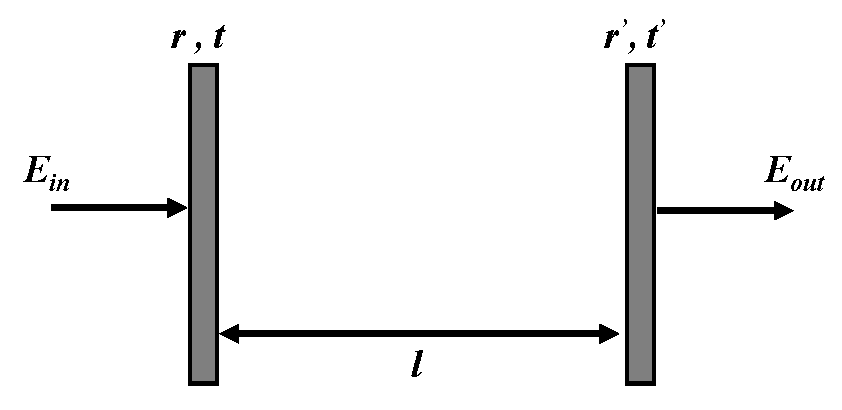
\includegraphics[width=0.6\textwidth]{figures/planar_fabry_perot.pdf}
    \caption{Sketch of a planar Fabry-Perot cavity.}
    \label{fig:planar_fabry-perot}
\end{figure}

Two planar slabs described by each their respective reflectivity \emph{r} and transmission \emph{t} are placed parallel and at a distance \emph{l} from eachother. The transmitted field $E_{out}$ is then given as a super position of all beams coupling into the cavity by $E_{in}$. In this way the Fabry-Perot cavity gives rise to so-called eigenstates\cite{Eichhorn} related to it's length \emph{l}, derived from considering the path difference between succesive parallel beams throught the cavity. The allowed modes inside the cavity are generally limited to ones which fulfill the identity\cite{Pedrotti}
\begin{equation}
    2 l \cos \theta = m \lambda.
    \label{eq:general_cavity_condition}
\end{equation}

Here $\theta$ is the incidence angle of the light coupling into the cavity, $\lambda$ is the wavelength of the light and $m = 1,2,3,...$ is a positive integer describing the order of the allowed mode. For the rest of this thesis it will be assumed that the laser couples into the cavity at normal incidence, meaning that $\theta = 0^{\circ}$ and thus $\cos \theta = 1$, as depicted in figure \ref{fig:planar_fabry-perot}.

\subsubsection{Transmission}

In order to determine the transmission throught the Fabry-Perot interferometer, we once again consider the configuration in figure \ref{fig:planar_fabry-perot}. It is further, initially, assumed that resonators are both lossless, such that
\begin{equation}
    |r|^2 + |t|^2 = |r^{\prime}|^2 + |t^{\prime}|^2 = 1.
    \label{eq:lossless_condition}
\end{equation}

This means that all losses, e.g. absorption, associated with the interaction between the field and the resonators are neglected. 

In order to formulate the transmitted field $E_{out}$ in terms of the ingoing one $E_{in}$, we first assume that the ingoing field can be described well by a plane-wave propagating in the z-direction
\begin{equation}
    E_{in} = E_{0,in} e^{ikz},
\end{equation}

where $k = 2 \pi / \lambda$ is the wave number and $E_{0,in}$ is the amplitude of the field. We then consider $E_{out}$ to be comprised of contributions for each roundtrip inside the cavity. This can be written as an infinite geometrical series given as
\begin{equation}
    \begin{split}
        E_{out} & = tt^{\prime} E_{0,in} e^{ikz} + tt^{\prime} E_{0,in} e^{ikz} rr^{\prime} e^{i\delta}\\&+ tt^{\prime} E_{0,in} e^{ikz} \left(rr^{\prime} e^{i\delta}\right)^2 + tt^{\prime} E_{0,in} e^{ikz} \left(rr^{\prime} e^{i\delta}\right)^3 + ...\\& = tt^{\prime} E_{0,in} e^{ikz} \sum^{\infty}_{m=0}\left( rr^{\prime}e^{i\delta} \right)^m
    \end{split}
    \label{eq:transmission_as_geometric_series}
\end{equation}
where $\delta = 2kl$. The first term of the series corresponds to a direct transmission through the cavity, and each term thereafter corresponds to the respective contribution to the transmission after the $m'th$ round trip. 

By evaluating the series it is seen that it indeed converges, and setting $z=l$ the final expression for the transmission through a planar Fabry-Perot cavity is found as
\begin{equation}
    E_{out} = E_{0,in}\frac{tt^{\prime} e^{i\delta /2}}{1 - rr^{\prime} e^{i\delta}}.
    \label{eq:fabry_perot_trans}
\end{equation}

\begin{figure}
    \centering
    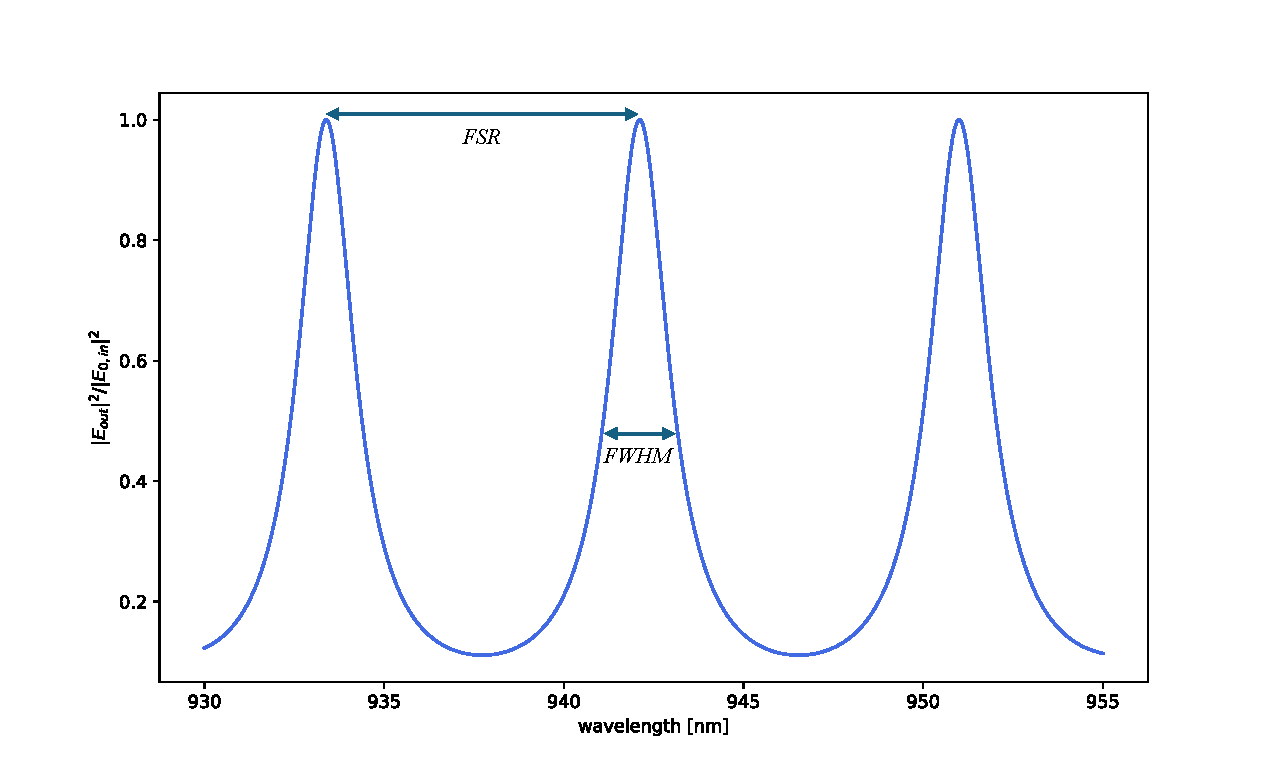
\includegraphics[width=0.6\textwidth]{figures/fabry_perot_example.pdf}
    \caption{Example of a Fabry-Perot cavity transmission (\~50um cavity length and $|r|^2 = 0.5$)}
    \label{fig:generic_fabry_perot}
\end{figure}

Figure \ref{fig:generic_fabry_perot} shows an example of the normalized transmission $|E_{out}|^2/|E_{0,in}|^2$ of an arbitrary Fabry-Perot cavity of length $l \approx 50 \mu m$ with reflectivity $|r|^2 = 0.5$. The two defining features marked on the figure are the \emph{Free Spectral Range (FSR)} and \emph{Full Width at Half Maximum (FWHM)}. As clearly depicted on the figure, the FSR is defined as the, in this case, spectral distance between two peaks in the spectra\footnote{The definition of the FSR is not limited to the distance between peaks in wavelength. As seen in eq. (\ref{eq:general_cavity_condition}) the cavity length and the resonant wavelengths are linearly dependent, and the length can thus just as well be varied resulting in a similar spectrum for the cavity transmission.}, while the FWHM is simply the linewidth of each peak. 

\subsubsection{Finesse}

Another important characteristic of an optical cavity is the so-called \emph{finesse} $\mathcal{F}$, which generally describes the quality of the cavity by the number of round trips the light makes on average before being transmitted. It can thus be said that the finesse corresponds to the order $m$ in the geometrical series describing the transmitted field $E_{out}$ in eq. (\ref{eq:transmission_as_geometric_series}), making the series, in any practical sense, finite.

There is a variety of ways one can obtain the finesse of a cavity. By examination of the spectrum one can find the finesse in terms of the FSR and FWHM, as seen in figure \ref{fig:generic_fabry_perot}, given as
\begin{equation}
    \mathcal{F} = \frac{FSR}{FWHM},
    \label{eq:finesse_FSR_FWHM}
\end{equation}
which indicates the resulting peaks of a cavity of higher finesse are narrower for the same FSR.

The finesse can also be expressed in terms of the reflectivity/transmission of the resonators of the cavity, as the defining phyisical action is that of the light either being transmittied from the cavity or not. The finesse in terms of $r$ and $t$, for both resonators, are given as
\begin{equation}
    \mathcal{F} = \frac{2 \pi}{1 - |r|^2 + 1 - |r^{\prime}|^2} = \frac{2 \pi}{|t|^2+|t^{\prime}|^2}.
    \label{eq:lossless_finesse}
\end{equation}

Figure \ref{fig:fabry_perot_trans} shows an example of the transmission spectrum of a high finesse cavity of reflectivity $|r|^2 = 0.9$ together with a low finesse cavity of reflectivity $|r|^2 = 0.3$. It is clearly seen that the linewidth of the high finesse cavity is much narrower than the low finesse case, which follows the relation shown in eq. (\ref{eq:finesse_FSR_FWHM}).

\begin{figure}[h!]
    \centering
    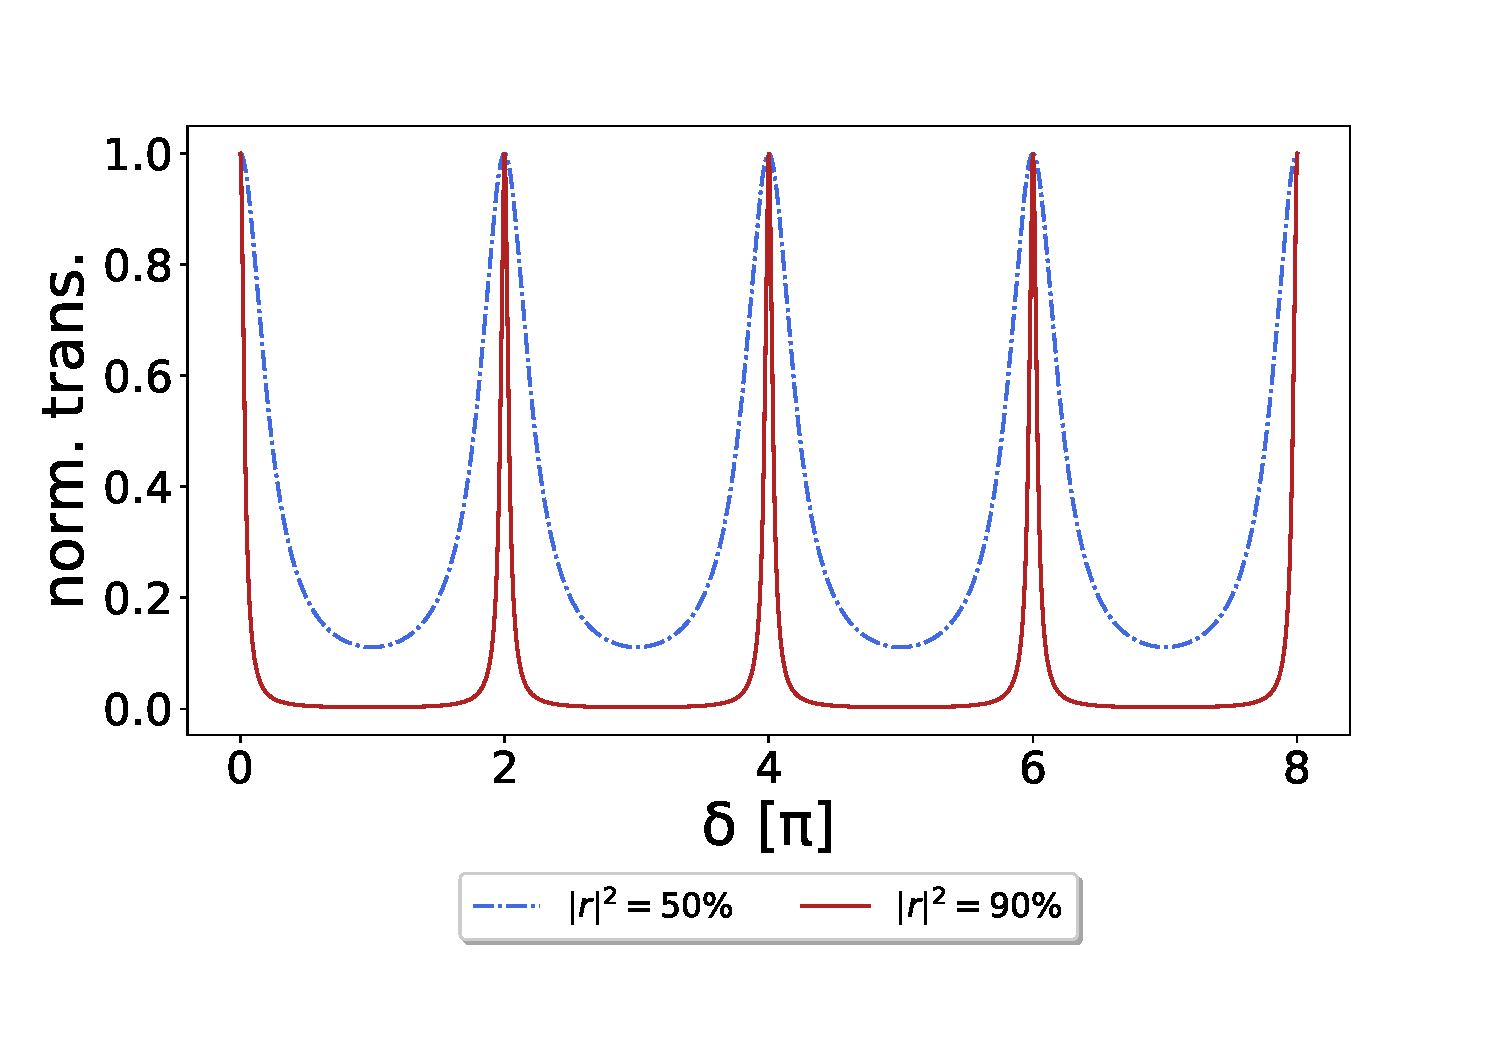
\includegraphics[width=0.6\textwidth]{figures/fabry_perot_high_and_low_finesse.pdf}
    \caption{Comparison of an arbitrary Fabry-Perot cavity of high and low finesse, respectively. The high finesse cavity and a reflectivity of $|r|^2 = 0.90$, while for the low finesse cavity $|r|^2 = 0.30$.}
    \label{fig:fabry_perot_trans}
\end{figure}


Eq. (\ref{eq:lossless_finesse}) however is only true for the case of a lossless cavity, i.e. when eq. (\ref{eq:lossless_condition}) is fulfilled. In practice, any cavity will have some amount of losses, which would have to be taken into account when calculating the finesse. When losses are present eq. (\ref{eq:lossless_condition}) instead generally reads
\begin{eqnarray}
    |r|^2 + |t|^2 + L + L^{\prime} = 1,
\end{eqnarray}
where $L$ and $L^{\prime}$ indicates the fractional losses of each resonator.

In this case the finesse would be given as 
\begin{equation}
    \mathcal{F} = \frac{2 \pi}{1-|r|^2 + 1 - |r^{\prime}|^2} = \frac{2 \pi}{|t|^2 + |t^{\prime}|^2 + L_{total}}.
\end{equation}

The effect on the transmission spectrum of a cavity with losses is that the level of the normalized transmission will not reach $1$, as some light is lost to i.g. absorption effects for each round trip of the cavity.

\subsubsection{Cavity length}

So far we have only considered effects that are independent of the length of the Fabry-Perot cavity, and by examining figure \ref{fig:fabry_perot_trans} it is seen that the only previously discussed feature that does not vary when changing the reflectivity and transmission (and by extension also the finesse) of the cavity, is the FSR. The FSR is defined as the distance between adjacent peaks of the transmission spectrum, and is given as
\begin{equation}
    FSR = \frac{c}{2nl},
    \label{eq:FSR_formula}
\end{equation}
where $c$ is the speed of light in vacuum, $n$ is the refractive index of the medium inside the cavity and $l$ is the length of the cavity. The inverse proportionality of the cavity length $l$ and the FSR is easily seen, and since the finesse is constant when varying the cavity length, the same must apply for the FWHM. Figure \ref{fig:fabry_perot_FSR_comparison} shows a comparison of the transmission through two Fabry-Perot cavities of length $100\mu m$ and $150 \mu m$, respectively. It is evident that the FSR depends on the cavity length, as $FSR_{100 \mu m} > FSR_{150 \mu m}$. It is also seen, that while the FSR becomes smaller with increasing cavity lengths, the linewidth does too, this is a consequence of the finesse $\mathcal{F}$ being constant in terms of the cavity length. 

\begin{figure}[h!]
    \centering
    \begin{subfigure}[b]{0.49\textwidth}
        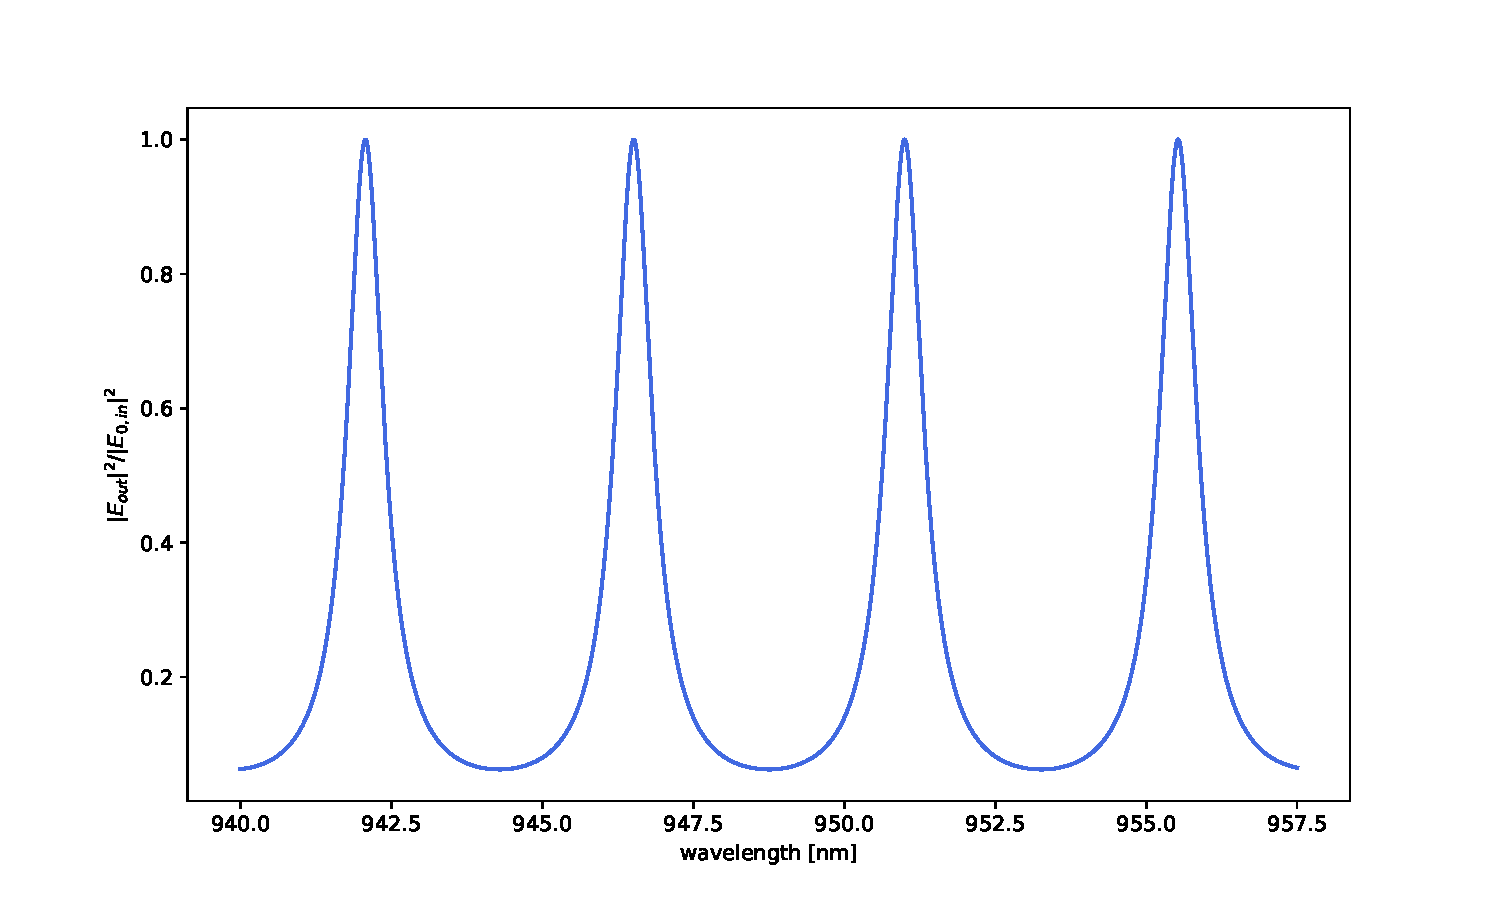
\includegraphics[width=\textwidth]{figures/100um_broadband_trans.pdf}
        \caption{$\sim 100 \mu m$ Fabry-Perot cavity transmission.}
    \end{subfigure}
    \begin{subfigure}[b]{0.49\textwidth}
        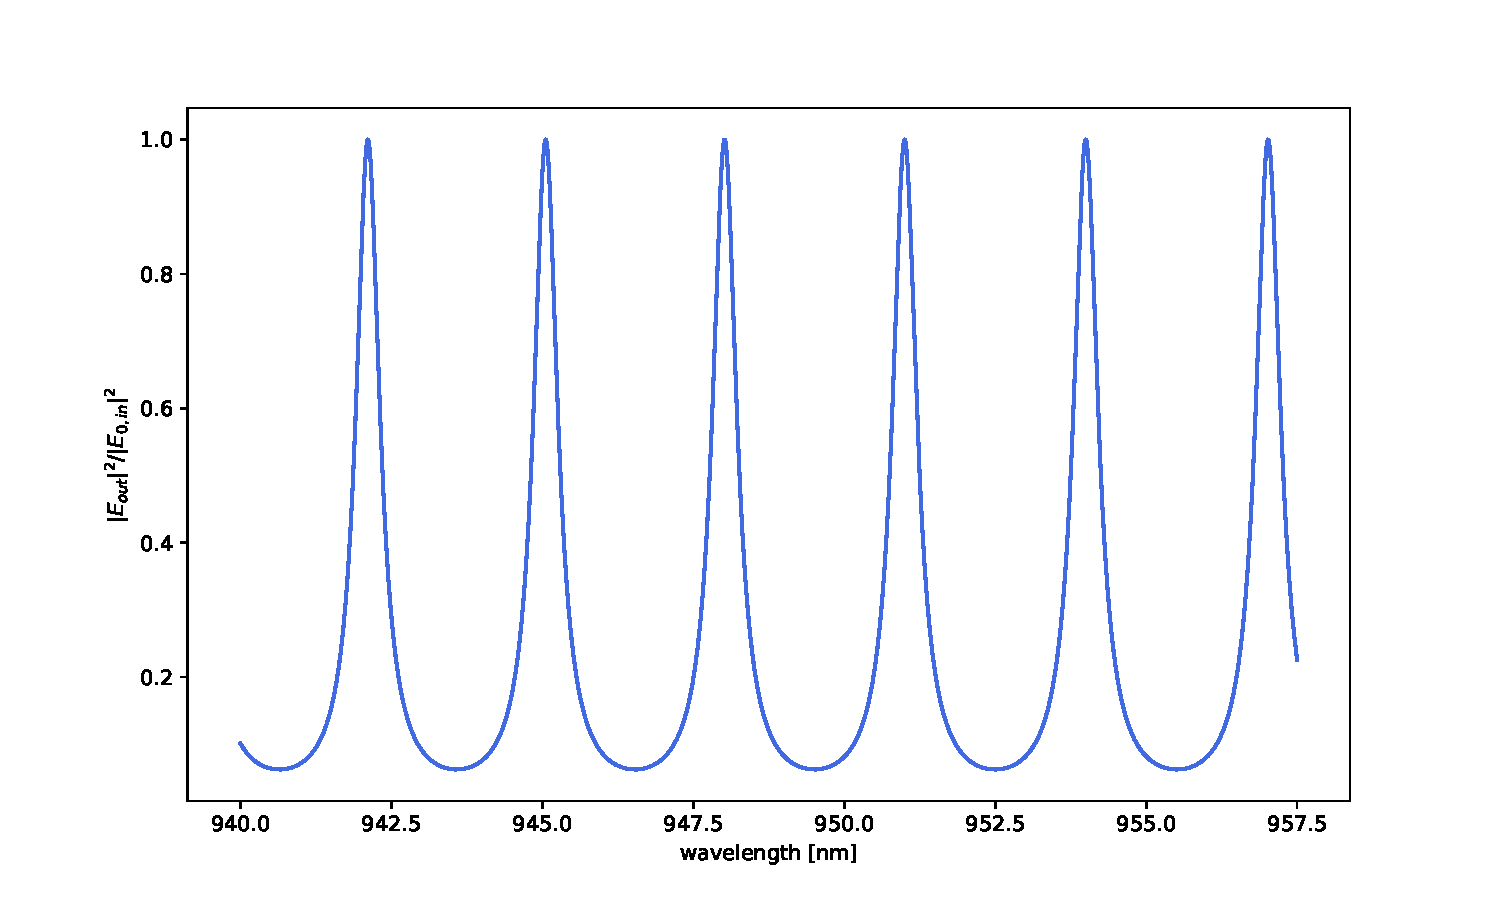
\includegraphics[width=\textwidth]{figures/150um_broadband_trans.pdf}
        \caption{$\sim 150 \mu m$ Fabry-Perot cavity transmission.}
    \end{subfigure}
    \caption{}
    \label{fig:fabry_perot_FSR_comparison}
\end{figure}


\subsubsection{The Fundamental Mode: A Gaussian Beam in the Large Waist Approximation}

In order to describe the allowed modes within an optical cavity, it is first assumed that a single-mode field is linearly polarized. We then consider solutions to the wave equation
\begin{equation}
    \nabla^2 \vec{E} = \frac{1}{c^2} \frac{\partial^2 \vec{E}}{\partial t^2},
\end{equation}
given as
\begin{equation}
    \vec{E} = E_0 (x,y,z) \vec{\epsilon} e^{i k z}. 
\end{equation}
Here $E_0(x,y,z)$ describes the electric field amplitude, $\vec{\epsilon}$ is denoted the polarization vector and $k=2 \pi / \lambda$ is the angular wave number of the field propagating along the z-axis. It is assumed that the electric field has a Gaussian transverse distribution\footnote{When this is the case, the laser is said to operate in the lowest possible mode denoted $TEM_{00}$. This implies the assumption of ideal lasing conditions.}.

This is almost the simplest description of the propagating field, however, as the spacial dependence of the field amplitude still might cause problems, we consider the range in which this can be neglected. 

It can be shown from the derivation of the Gaussian distribution that the waist of the beam $w(z)$, which depends on the spacial coordinate in the direction of propagation, can be described as \cite{Eichhorn}
\begin{equation}
    w(z) = w_0 \sqrt{1 + \left(\frac{z}{z_R}\right)^2},
    \label{eq:gaussian beam waist}
\end{equation}
where $z$ is the distance from focus, $w_0$ is the beam waist at focus and $z_R$ is the so-called \emph{Rayleigh range}. The Rayleigh range describes the range in which the beam diverges slowly, whereas after this has been surpassed, the beam will begin to diverge more rapidly. By quick inspection of eq. (\ref{eq:gaussian beam waist}) it is seen that
\begin{equation}
    w(z) = 
    \begin{cases}
        w_0, & \mbox{for } z=0 \\
        w_0\sqrt{2}, & \mbox{for } z=z_R,
    \end{cases}
\end{equation}
which shows that the beam waist diverges no more than by a factor of $\sqrt{2}$ from the optimal case, for $0\leq z \leq z_R$. Considering the case where $z \neq 0$ but however much smaller than the Rayleigh range $z_R$, we can further inspect eq. (\ref{eq:gaussian beam waist}) and find that this leads to negligible changes in the waist of the beam. Specifically, it can fairly easily be seen that
\begin{equation}
    \left(\frac{z}{z_R}\right)^2 \approx 0, \: \text{  for } z << z_R
\end{equation}
which in turn leads to 
\begin{equation}
    w(z) \approx w_0.
\end{equation}

The Rayleigh range can be written as \cite{Pedrotti}
\begin{equation}
    z_R = \frac{\pi w_0^2}{\lambda},
    \label{eq:Rayleigh range}
\end{equation}
which, through the exponential dependence on $w_0$, shows that a large beam waist will result in a long Rayleigh range. As an example, consider a beam of waist $w_0 = 200 \mu m$ and wavelength $\lambda = 950 nm$. This would result in a Rayleigh range of $z_R=13.23 cm$. 

Finally we can conclude, that any optical cavity, for which the total distance travelled inside the cavity\footnote{For any optical cavity the incident light will travel a distance inside the cavity according to, not only the length of the cavity, but also the amount of round trips the light makes when confined inside the cavity.}, is significantly shorter than the Rayleigh range of the incident beam, the spacial dependence of the field amplitude inside the cavity is negligible, and the fundamental mode can be described simply by a linearly polarized plane wave
\begin{equation}
    \vec{E} = E_0 \vec{\epsilon} e^{ikz}.
\end{equation}
This is often referred to as the \emph{large waist approximation} of a Gaussian beam, due to the dependence on $w_0$ of eq. (\ref{eq:Rayleigh range}).